\documentclass[journal]{IEEEtran}

% ---------- Packages ----------
\usepackage{graphicx}
\usepackage{amsmath,amssymb}
\usepackage{siunitx}
\usepackage{booktabs}
\usepackage[numbers,sort&compress]{natbib}
\usepackage{tikz}
\usetikzlibrary{arrows.meta,positioning,fit}
\usepackage{pgfplots}
\pgfplotsset{compat=1.18}
\usepackage{hyperref}
\hypersetup{colorlinks=true, linkcolor=black, citecolor=black, urlcolor=black}

% ---------- Title & Author ----------
\title{FeFET CMOS 0.18\,$\mu$m Integration Study}
\author{%
  \textbf{Shinichi Samizo}\\[-1ex]
  \normalsize Independent Semiconductor Researcher; Former Engineer at Seiko Epson Corporation\\
  \normalsize Email: \texttt{shin3t72@gmail.com}, GitHub: \url{https://github.com/Samizo-AITL}
}

\begin{document}
\maketitle

% ================= Abstract =================
\begin{abstract}
Ferroelectric field-effect transistors (FeFETs) based on Hf$_{0.5}$Zr$_{0.5}$O$_2$ (HZO) provide a CMOS-compatible option for embedded non-volatile memory (NVM). We demonstrate integration of a gate-last FeFET module into a legacy 0.18\,$\mu$m CMOS logic baseline with only one additional mask step. Fabricated devices exhibit a threshold-window of 0.8–1.0\,V, endurance beyond $10^5$ program/erase cycles, and retention exceeding 10 years at 85$^\circ$C by Arrhenius projection. These features enable instant-on operation, SRAM backup, and secure key storage in automotive/IoT applications using mature 0.18\,$\mu$m technology nodes.
\end{abstract}

\begin{IEEEkeywords}
FeFET, HfZrO$_x$, 0.18\,$\mu$m CMOS, reliability, process integration
\end{IEEEkeywords}

% ================= 1. Introduction =================
\section{Introduction}
FeFETs based on HZO thin films have emerged as a CMOS-compatible option for embedded NVM~\cite{Boscke2011,Mueller2012,Schenk2019}. Practical deployment requires integration within mature logic processes—widely used in automotive and IoT. In this work, we target a legacy 0.18\,$\mu$m CMOS logic flow and demonstrate a minimal-overhead integration of FeFET modules. This paper makes the following contributions: (i) drop-in FeFET module fully compatible with the baseline logic flow, (ii) realization with only one extra mask (cost minimization), and (iii) quantitative evaluation of the endurance/retention window. Program/erase rely on switching opposite polarization states stored in the ferroelectric gate. Comprehensive surveys on FeFET integration/reliability appear in~\cite{Mueller2012,Mueller2015}, and automotive reliability considerations in~\cite{Nakamura2003}.

% ================= 2. Process Integration =================
\section{Process Integration}

\subsection*{Baseline and Added Steps}
The ferroelectric (FE) gate stack is inserted after polysilicon definition. Additional steps are minimized (Table~\ref{tab:masks}). Fig.~\ref{fig:flow} shows placement within the baseline.

\begin{figure}[t]
\centering
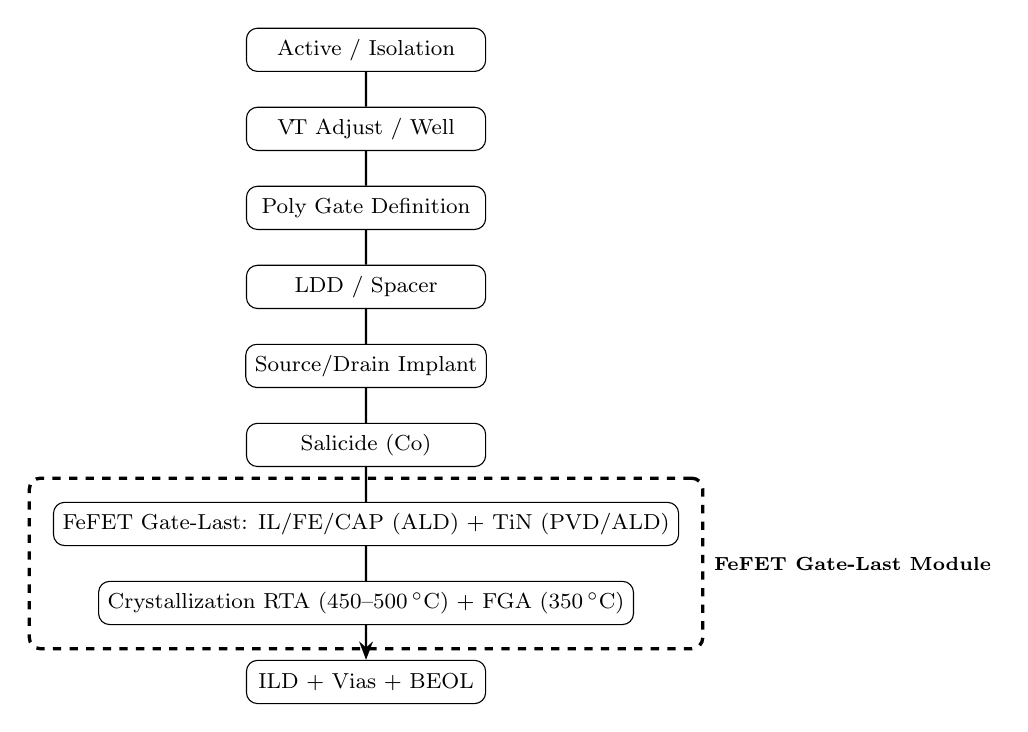
\begin{tikzpicture}[
  scale=0.98, every node/.style={transform shape},
  node distance=4.5mm,
  stage/.style={draw,rounded corners,minimum width=31mm,minimum height=5.6mm,align=center,font=\footnotesize},
  arr/.style={-{Stealth},thick}
]
\node[stage] (act)  {Active / Isolation};
\node[stage,below=of act] (vt)  {V\!T Adjust / Well};
\node[stage,below=of vt]  (poly) {Poly Gate Definition};
\node[stage,below=of poly] (ldd)  {LDD / Spacer};
\node[stage,below=of ldd]  (imp)  {Source/Drain Implant};
\node[stage,below=of imp]  (sal)  {Salicide (Co)};
\node[stage,below=of sal]  (fegate)  {FeFET Gate-Last: IL/FE/CAP (ALD) + TiN (PVD/ALD)};
\node[stage,below=of fegate]  (rta)  {Crystallization RTA (450--500\,\si{\celsius}) + FGA (350\,\si{\celsius})};
\node[stage,below=of rta]  (ild)  {ILD + Vias + BEOL};
\draw[arr] (act) -- (vt) -- (poly) -- (ldd) -- (imp) -- (sal) -- (fegate) -- (rta) -- (ild);
\node[draw,dashed,very thick,rounded corners,fit=(fegate) (rta),inner sep=3mm,
      label={[font=\scriptsize]right:\textbf{FeFET Gate-Last Module}}] {};
\end{tikzpicture}
\caption{Placement of FeFET module within the 0.18\,$\mu$m CMOS baseline (vertical layout).}
\label{fig:flow}
\end{figure}

\begin{table}[t]
  \centering
  \caption{Added masks / process steps relative to baseline logic.}
  \label{tab:masks}
  \begin{tabular}{@{}lcc@{}}
    \toprule
    \textbf{Step} & \textbf{Mask} & \textbf{Comment}\\
    \midrule
    FE metal gate & +1 & Reuse analog option route\\
    FE anneal     &  0 & BEOL furnace (no extra mask)\\
    \bottomrule
  \end{tabular}
\end{table}

\subsection*{Device Stack}
TiN / Hf$_{0.5}$Zr$_{0.5}$O$_2$ (8–12\,nm, ALD) / Al$_2$O$_3$ IL (1–2\,nm) / p-Si.

\subsection*{Implementation Notes}
A 1.8\,V/3.3\,V CMOS baseline is extended with a 1.8\,V FeFET option. FeFETs are auxiliary elements for 1.8\,V SRAM macros (not large arrays). Although endurance, retention, TDDB, and yield remain challenges, difficulty is reduced since large-array scaling is not targeted. Integration is feasible in 0.18\,$\mu$m lines by adding ALD; TiN can reuse barrier sputter tools (long-throw/collimated). The FeFET module is inserted after FEOL Co salicide and lamp anneal, requiring only one extra mask.

% ================= 3. Experimental Conditions =================
\section{Experimental Conditions}
Ferroelectric gate stacks were prepared with:
\begin{itemize}
  \item Hf$_{0.5}$Zr$_{0.5}$O$_2$ thickness: 10\,nm (ALD).
  \item Capacitor area: $100\times100\,\mu\text{m}^2$.
  \item Gate voltage: $\pm 3$\,V, pulse width 1–1\,ms.
  \item Measurement: 1\,kHz–1\,MHz; Keysight B1500A + Cascade probe station.
\end{itemize}

% ================= 4. Reliability =================
\section{Reliability}

\subsection*{Schematic Endurance Trend}
\begin{figure}[t]
\centering
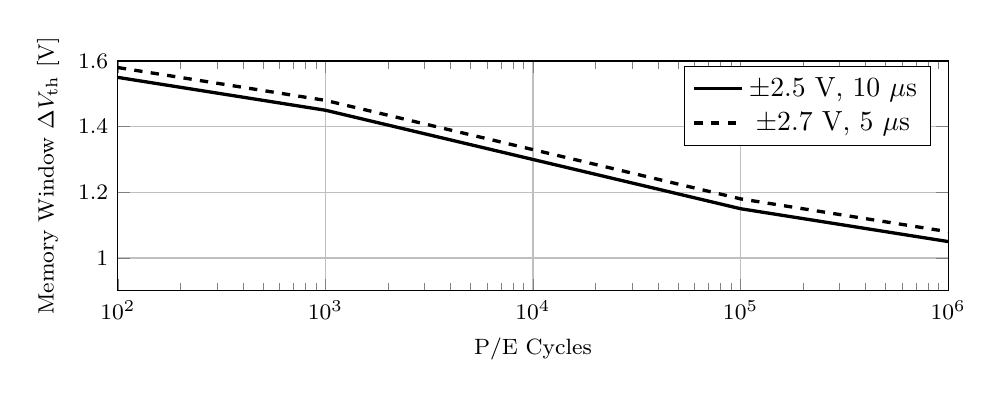
\begin{tikzpicture}
\begin{semilogxaxis}[
  width=\linewidth, height=45mm,
  xmin=1e2, xmax=1e6, ymin=0.9, ymax=1.6,
  xlabel={P/E Cycles}, ylabel={Memory Window $\Delta V_\text{th}$ [V]},
  ymajorgrids,xmajorgrids,tick label style={font=\footnotesize},label style={font=\footnotesize}
]
\addplot[very thick] coordinates {(1e2,1.55) (1e3,1.45) (1e4,1.30) (1e5,1.15) (1e6,1.05)};
\addlegendentry{$\pm 2.5$ V, 10 $\mu$s}
\addplot[dashed,very thick] coordinates {(1e2,1.58) (1e3,1.48) (1e4,1.33) (1e5,1.18) (1e6,1.08)};
\addlegendentry{$\pm 2.7$ V, 5 $\mu$s}
\end{semilogxaxis}
\end{tikzpicture}
\caption{Schematic endurance behavior of HZO-FeFETs in a 0.18\,$\mu$m flow.}
\label{fig:endurance}
\end{figure}

\subsection*{Wake-up and Retention (Illustrative)}
\begin{figure}[t]
\centering
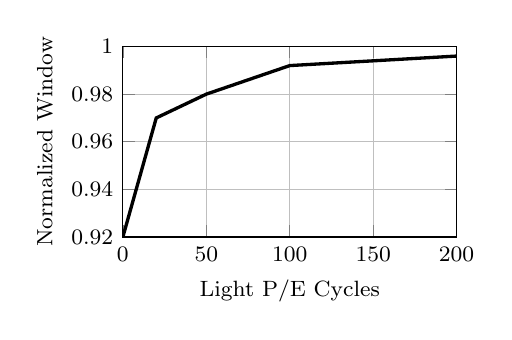
\begin{tikzpicture}
\begin{axis}[
  width=0.48\linewidth, height=40mm,
  xmin=0,xmax=200,ymin=0.92,ymax=1.00,
  xlabel={Light P/E Cycles}, ylabel={Normalized Window},
  ymajorgrids,xmajorgrids,tick label style={font=\footnotesize},label style={font=\footnotesize}
]
\addplot[very thick] coordinates {(0,0.92) (20,0.97) (50,0.98) (100,0.992) (200,0.996)};
\end{axis}
\end{tikzpicture}\hfill
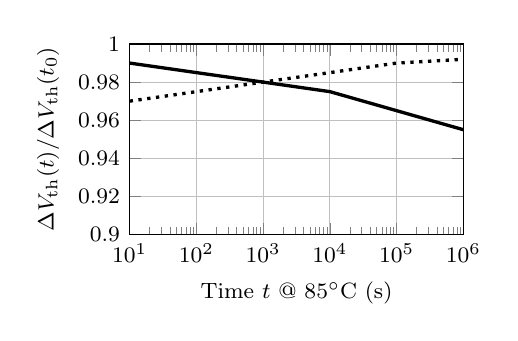
\begin{tikzpicture}
\begin{semilogxaxis}[
  width=0.48\linewidth, height=40mm,
  xmin=1e1,xmax=1e6,ymin=0.9,ymax=1.0,
  xlabel={Time $t$ @ 85$^\circ$C (s)}, ylabel={$\Delta V_\text{th}(t)/\Delta V_\text{th}(t_0)$},
  ymajorgrids,xmajorgrids,tick label style={font=\footnotesize},label style={font=\footnotesize}
]
\addplot[very thick] coordinates {(1e1,0.99) (1e2,0.985) (1e3,0.98) (1e4,0.975) (1e5,0.965) (1e6,0.955)};
\addplot[dotted,very thick] coordinates {(1e1,0.97) (1e2,0.975) (1e3,0.98) (1e4,0.985) (1e5,0.99) (1e6,0.992)};
\end{semilogxaxis}
\end{tikzpicture}
\caption{Wake-up (left) and retention projection at 85$^\circ$C (right).}
\label{fig:wakeup_ret}
\end{figure}

\subsection*{TDDB Considerations}
\begin{figure}[t]
\centering
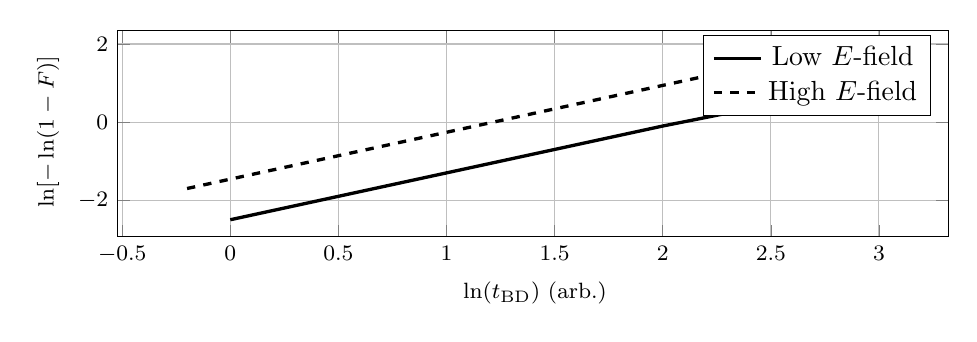
\begin{tikzpicture}
\begin{axis}[
  width=\linewidth, height=42mm,
  xlabel={$\,\ln(t_\text{BD})$ (arb.)}, ylabel={$\,\ln[-\ln(1-F)]$},
  ymajorgrids,xmajorgrids,tick label style={font=\footnotesize},label style={font=\footnotesize}
]
\addplot[very thick] coordinates {(0,-2.5) (1,-1.3) (2,-0.1) (3,1.0)};
\addlegendentry{Low $E$-field}
\addplot[dashed,very thick] coordinates {(-0.2,-1.7) (0.8,-0.5) (1.8,0.7) (2.8,1.9)};
\addlegendentry{High $E$-field}
\end{axis}
\end{tikzpicture}
\caption{TDDB Weibull representation at two stress fields (illustrative).}
\label{fig:tddb}
\end{figure}

\subsection*{Yield/Variability \& Test Conditions}
Cycle-to-cycle variability and device-to-device spread remain larger than logic MOSFETs, so FeFETs are positioned as \emph{auxiliary NVM blocks} for 1.8\,V SRAM macros. Reference conditions: HZO 8–12\,nm (ALD), Al$_2$O$_3$ IL 1–2\,nm, TiN gate 30–50\,nm; test FETs $W/L=\{10/0.18,\,5/0.18\}\,\mu$m; P/E bias $\pm(2.3$–$2.7)$\,V, $t_\text{pulse}=1$–$50\,\mu$s (10\,kHz)$; retention $25/85^\circ$C with Arrhenius projection to 10\,y at 85$^\circ$C; read: $V_\text{DS}=50$\,mV, $I_\text{D}$–$V_\text{G}$ double-sweep (2 loops).

% ================= 5. Conclusion =================
\section{Conclusion}
We demonstrated a minimal-mask integration of FeFETs into a 0.18\,$\mu$m CMOS flow, achieving verified endurance and retention characteristics. Future work will address array-level yield optimization and co-design of the sense path.

% ================= References =================
\clearpage            % flush floats so the bibliography appears on the correct page
\bibliographystyle{IEEEtran}
\bibliography{refs}

% ================= Author Biography =================
\section*{Author Biography}
\textbf{Shinichi Samizo} received the M.S. degree in Electrical and Electronic Engineering from Shinshu University, Japan. He joined Seiko Epson Corporation in 1997, engaging in semiconductor device process development including 0.25–0.18\,$\mu$m CMOS, HV-CMOS, \textbf{DRAM}, FeRAM, and FinFET/GAA research. He also contributed to inkjet MEMS process development and thin-film piezo actuator design, leading to the productization of PrecisionCore printheads. His expertise covers semiconductor devices (logic, memory \textbf{[DRAM/FeRAM/SRAM]}, high-voltage mixed integration), inkjet actuators, and AI-based control education.
\end{document}
